\documentclass{article}
\usepackage{amsmath}
\usepackage[pdftex]{graphicx}

\begin{document}
\author{Tobias Reisch}
\title{Report on readAFM}
\maketitle

\section{The Project}

The goal of this project was explore the possibilities of using Machine Learning to analyze data obtained from Non Contact Atomic Force Microscopy.

This report contains a brief description of the most important steps in the project, especially
\begin{itemize}
\item How to generate the input data.
\item How to generate the labels.
\item How the Neural Net was built.
\item Highlights of the Results.
\end{itemize}

\newpage
\section{Input}

Machine Learning usually needs a lot of training data to work. In our case this would be measured frequency shifts or forces from AFM experiments. Since there exists no database of labeled AFM 'images' we decided to use simulated data. We used the \emph{MechAFM} program developed in our group based on \cite{hapala2014, hamalainen2014} to generate three dimensional datasets filled with force values. The inputs for \emph{MechAFM} consist of a xyz-file, a file specifying the potentials to use for the molecular dynamics simulation and a set of parameters. The values used that are different from the default parameters are:

\begin{center}
\begin{tabular}{|c|c|}
\hline area & 8 {\AA} x 8 {\AA} \\ 
\hline zlow & position of topmost atom + 4 {\AA} \\ 
\hline zhigh & zlow + 4 {\AA} \\ 
\hline dx,dy,dz & 0.2 {\AA} \\ 
\hline 

\end{tabular} 
\end{center}

The output of \emph{MechAFM} consists of the force acting on the tip in z-direction, the angle of the CO-molecule and the displacement of the tip atom. We only keep the force in z-direction, which is compiled to a \emph{Numpy} array and stored in a hdf5-container. Additionally we store data like the name string, the position of the atoms, the array-size, etc. as attributes in the hdf5-file. The data is separated randomly into a training and a validation set, with roughly a 80:20 splitting.

% Maybe mention the structure of the hdf5 files?

\newpage

\section{Labels}
For this large amount of simulated AFM data, we would like to automatically generate labels. This step should be done very carefully, because it will also determine what the Neural Net will output. If we assign labels containing more information about the molecule than there is in the AFM data, the NN will not be able to train successfully, on the other hand, we want to get as much out of it as possible. We could, of course, ask the NN to predict the chemical sum formula for the molecule, but for this sort of analysis, there are already many different techniques available. And it is the big strength of atomic resolution AFM, that the spatial structure of the molecules can be determined. So the labels are a balance between extracting as much information as possible, determining the spatial structure of the molecule and bringing it into a form that is useful for the NN to learn. I.e. it is easier to ask for a constant length output, than for a variable length output (i.e. the NN outputs a list of atom positions).

For our case we decided it would be best (at the beginning) to produce a xy-map with values that are large when there is an atom at that position and zero otherwise. A projection of the atoms coordinates to the xy-plane, but replacing the atoms with Gaussians scaled according to the covalent radius of the element. The formula for the Gaussians looks like this:

\begin{equation}
amp(element) = amp_0 * \frac{covalent radius(element)}{covalen radius(carbon)}
\end{equation}
\begin{equation}
\sigma = \sigma_0 * \frac{covalent radius(element)}{covalen radius(carbon)}
\end{equation}
\begin{equation}
signal(\vec{r}) = amplification*\exp(-\frac{(\vec{r}-\vec{r_0})^2}{\sigma^2})
\end{equation}

Where $amp_0$ and $\sigma_0$ are the input parameters and $\vec{r_0}$ is the position of the atom. To take into account, that atoms that are further away from the tip than others are less visible, we interpret the Gaussians as Gaussians in three dimensions and evaluate them at every point in the xy-plane at the height (z-value) of the topmost atom. It turned out to be beneficial to use different values for $\sigma$ in the xy-plane and in the z-direction. See also fig \ref{fig:gaussians}.

 \begin{figure}[htbp]
 	\begin{center}
 		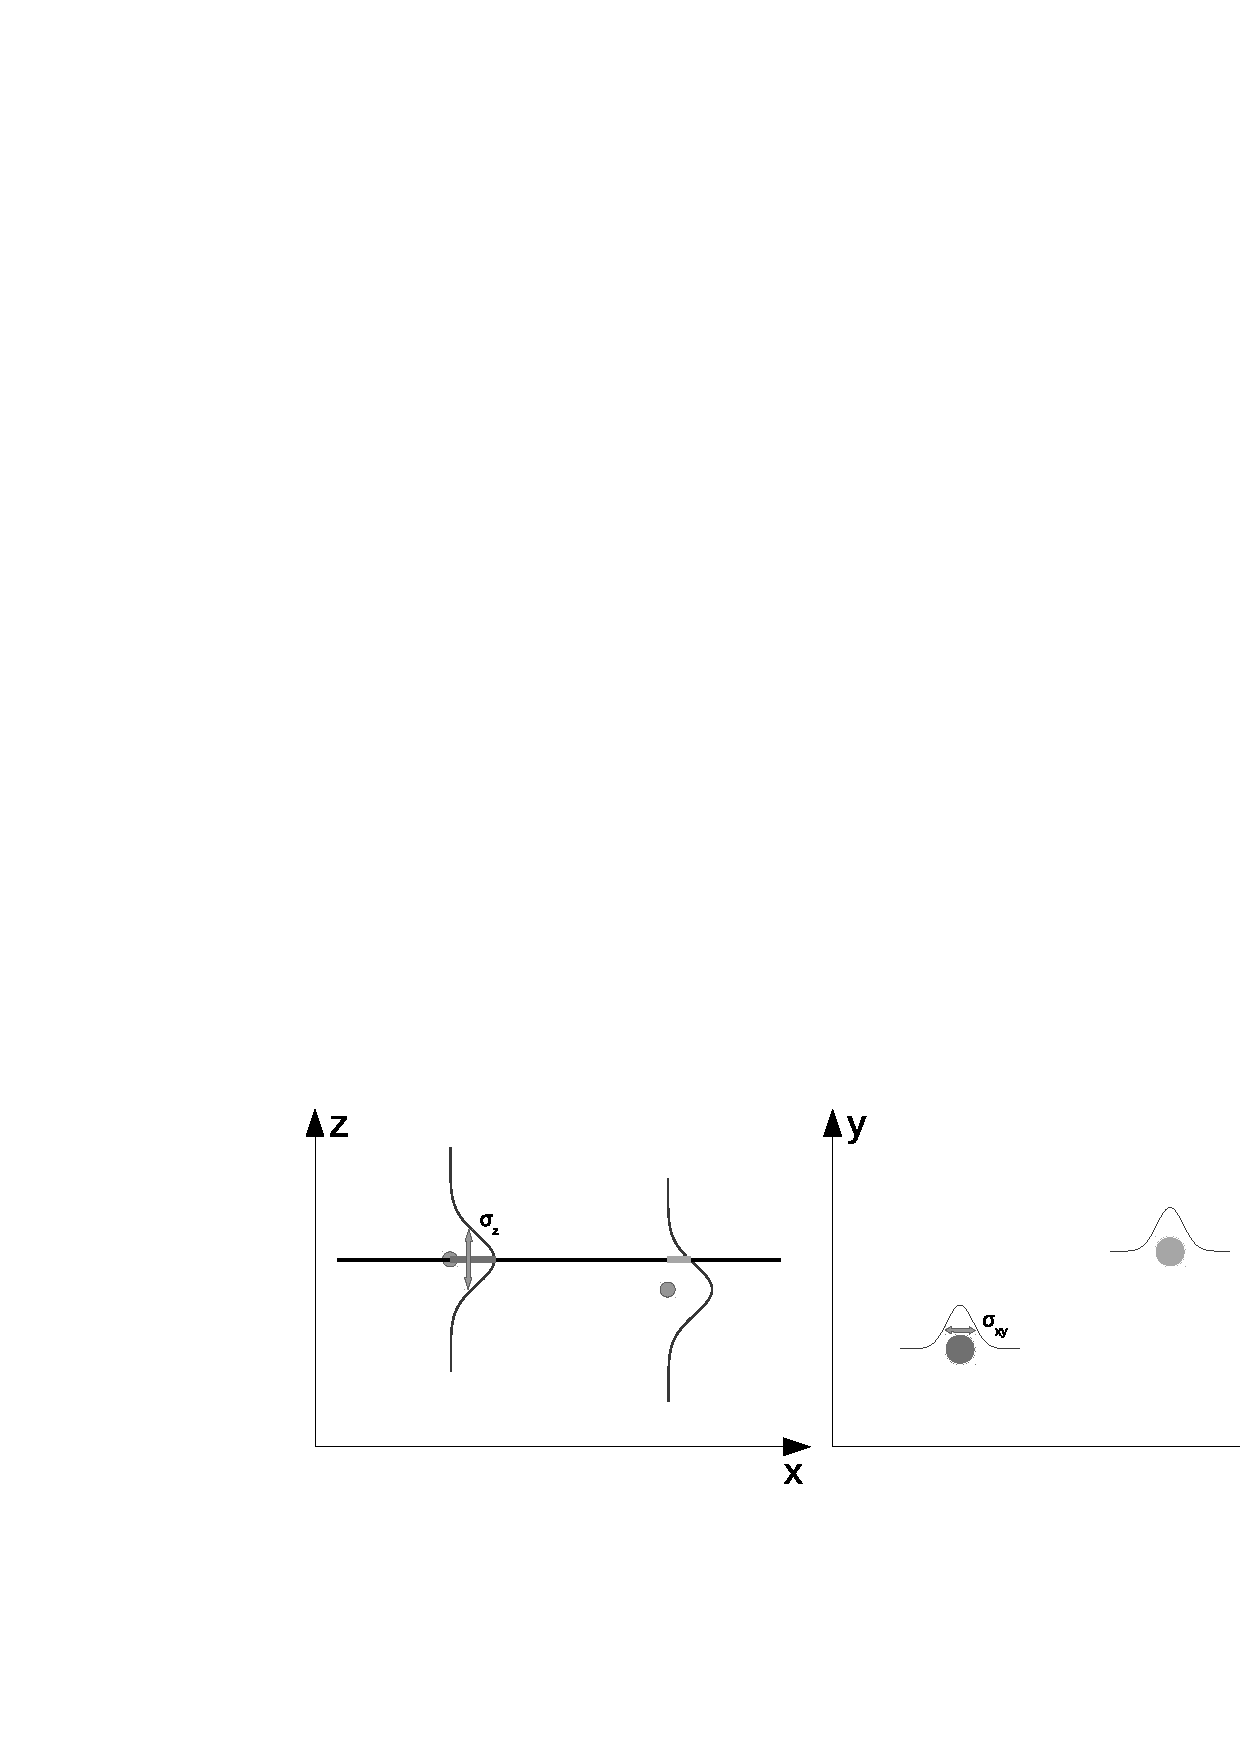
\includegraphics[width=12cm]{figs/gaussians.png}
 		\caption{Schematic explanation of the labelling process.}
 		\label{fig:gaussians}
 	\end{center}
 \end{figure}

It is crucial to choose $\sigma_z$ carefully, since for a to large value all the atoms would appear in the labels whereas the atoms far away from the tip would not appear in the force images, on the other hand for a too small $\sigma_z$ only the topmost atom would be included in the labels, while in the force curves also lower lying atoms appear.

To determine $sigma_z$ rigorously we used a concept known from Information Theory, Mutual Information, which has recently been introduced to our group \cite{MIestimator}. The idea is that Mutual Information is large when two distributions contain similar information and small else. We calculated MI vs. $\sigma_z$ curves \ref{fig:MIcurve}, and they show a clear maximum.

 \begin{figure}[htbp]
 	\begin{center}
 		\includegraphics[width=12cm]{figs/Mutual_information-fullDB-k5_amp10_n1000.png}
 		\caption{Mutual Information vs. $\sigma_z$ for three dimensional molecules in random orientations. The spread can be explained by the fact, that the 1000 samples to calculate MI at every point were drawn randomly every time.}
 		\label{fig:MIcurve}
 	\end{center}
 \end{figure}



\newpage
\section{CNN}
In recent years there have been great advances with deep learning and Convolutional Neural Nets \cite{krizhevsky2012imagenet}. We try to apply this to our task of analyzing AFM data. For our task using a CNN seems feasible, for several reasons:
\begin{itemize}
\item Its translational invariance allows (theoretically) to use the same filters for different image sizes.
\item The use of filters of a particular size can account for the flexibility of the CO-molecule at the end of the tip.
\end{itemize}

 \begin{figure}[htbp]
 	\begin{center}
 		\includegraphics[width=12cm]{figs/minimal_CNN.png}
 		\caption{Our NN}
 		\label{fig:NNstruct}
 	\end{center}
 \end{figure}

Our dataset can be imagined as a tensor of order 4, three indices for the spatial degrees of freedom (x,y,z) and one index for the "input channels", when treating color images this number is three, for the color three channels RGB. In our case there is just one input channel, the forces. In the first convolutional layer, this tensor is convolved with 16 filters of the size 0.8 x 0.8 x 0.8{\AA}, the convolution preserves the spatial size of the tensor, but the number of "channels" grows to 16. After applying the hyperbolic tangent function as nonlinearity, we repeat the convolution step with 32 filters.

After the 3D convolutions preserved the order of the tensor, now we want to reduce it to a two dimensional image. To achieve this, we flatten the axes of the tensor corresponding to z and the channels and use them as input to a fully connected layer. After the fully connected layer we apply a rectified linear (ReLU) operation as nonlinearity and we receive the output. To stay with the language of tensors: Now we have a tensor of order three, two spatial degrees of freedom and one output channel. The size of the spatial axes is conserved. For a schematic explanation see fig. \ref{fig:NNstruct}.

For this Neural Net the filters of the convolution and the weights and biases can be trained with gradient descent. We used stochastic training with the Adam Optimizer \cite{kingma2014adam}, which was especially designed for stochastic training. 

The accuracy and trainability of this Neural Net can be changed in a several ways: By changing the filter size and number in the convolutions, using different sized fully connected layers (a FC layer with 64 neurons already works, but using larger FC layers improves the result drastically!) and of course adding more layers. The effect of these changes will be discussed in the next section.


\newpage
\section{Results}

\bibliographystyle{unsrt}
\bibliography{readAFM}

\end{document}



